\documentclass[../main.tex]{subfile}
\graphicspath{{\subfix{../images}}}
\begin{document}

我们的目标是借助卷积网络的金字塔特征层级,它有从低到高的语义层级,并构建一个在各处都有高层级语义的特征金字塔。最终的\textit{特征金字塔网络}是通用目的的,在这片文章中我们专注于滑动窗口候选生成(候选区域网络,RPN)和基于区域的检测器(Faster R-CNN)。我们也在第6章中将FPN推广到分割候选。

我们的方法将任意大小的单一尺度图片作为输入,并在多个尺度通过全卷积的方式输出相应尺度的特征图。这个过程与骨干卷积网络架构(例如,\cite{19,36,16})是独立的,在这篇文章中我们展示了使用ResNets\cite{resnet}的结果。正如后面将要介绍的,我们的金字塔构建过程涉及一个自底向上的通路、一个自顶向下的通路和旁路连接。

\paragraph{自底向上通路。}自底向上的通路是骨干网卷积络的前向传播计算,它会计算一个由以缩放步长为2变化的各个尺度的特征组成的特征层级。通常会存在多个产生相同大小的输出特征图的层,我们称这些层在同一个\textit{阶段(stage)}。对于我们的特征金字塔,我们为每一个阶段定义一个金字塔层级。我们选择每个阶段最后一层的输出作为我们对于这个阶段的参考。由于每一个阶段最深的层应该有最强的特征,所以这个选择是自然的。

特别的,对于ResNets\cite{resnet}我们使用了每一个阶段的最后一个残差模块的特征激活输出。对于conv2, conv3, conv4和conv5的输出,我们将这些最后的残差模块的输出记为$\{C_2, C_3,C_4,C_5\}$,并且它们对于输入图像的步长为$\{4, 8, 16, 32\}$个像素。由于conv1巨大的内存占用,我们没有将它包括在金字塔内。

\paragraph{自顶向下通路和旁路连接。}自顶向下通路通过对空间更加粗糙但是语音更强的来自金子塔更高层级的特征进行上采样,仿佛得到了更高分辨率的特征。这些特征接着会被来自自底向上通路的特征经过旁路连接增强。每个旁路连接将会合并来自自底向上通路和自顶向下通路中有相同空间大小的特征图。自底向下的特征图的语义层级更低,但是由于它被下采样的次数更少,所以它的激活被更加准确地定位。

\begin{figure}[bh]
    \centering
    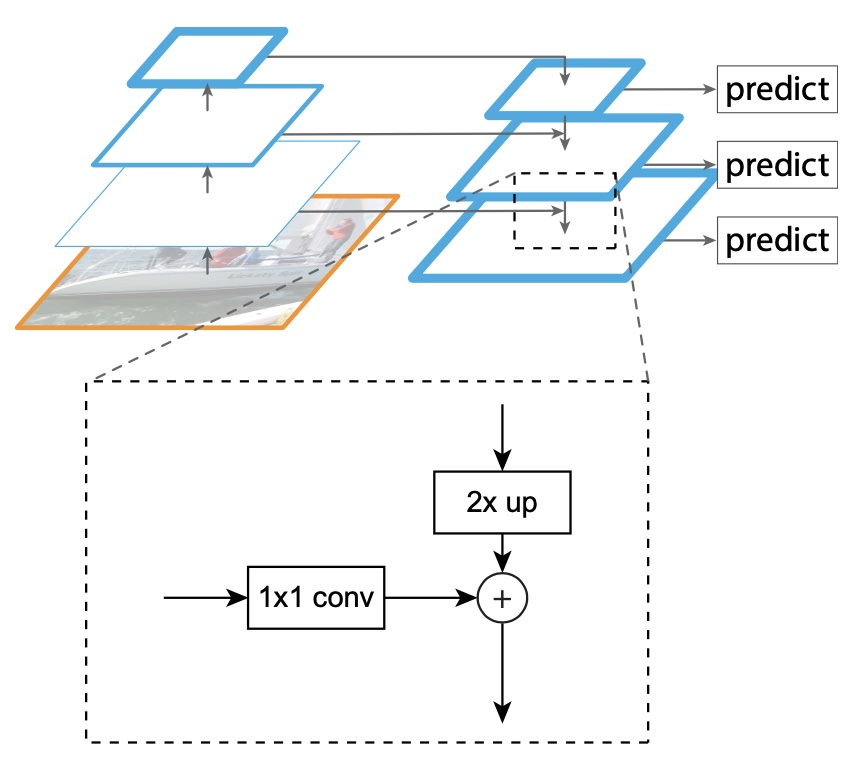
\includegraphics[width=.8\textwidth]{img3.png}
    \caption{一个展示了旁路连接和自顶向下通路的构造模块,通过相加合并。}
    \label{fig:img1}
\end{figure}

图\ref{fig:img3}展示了构建我们的特征图的构造模块。有了更粗糙分辨率的特征图,我们将它的空间分辨率以系数2进行上采样(出于简便使用最近邻上采样)。接着上采样得到的特征图与对应的自底向上通路中的特征图(它会经历一个$1\times 1$卷积层来减少通道维度)通过对应元素相加的方式合并。这个过程将会被迭代只到最好分辨率的特征图被生成。为了开始迭代,我们简单地在$C_5$上依附一个$1\times 1$卷积层来生成最粗糙的特征图。最终,我们在每一个合并得到的特征图上添加一个$3\times 3$卷积来生成最终的特征图,卷积被用来减弱上采样的对齐影响。这个最终特征图的集合被称为$\{P_2,P_3,P_4,P_5\}$,对应于分别有相同空间大小的$\{C_2,C_3,C_4, C_5\}$。

由于在传统的特征化图片金字塔中,金字塔的所有层级使用共享的分类器/回归器,所以我们在所有特征图中固定了特征维度(通道数,记为$d$)。我们在这篇文章中设置$d=256$,因此所有额外的卷积层输出通道数都为256。这些额外层没有非线性,我们经验性地发现这影响并不大。

简便性是我们设计的中心,同时我们发现我们的模型对于多个不同的设计选择具有鲁棒性。我们使用更加精细的模块(例如,使用多层残差模块\cite{resnet}作为连接)进行了实验,并观察到了些微更好的结果。设计更好的连接模型不是本文的关注点,所以我们选择了如上所述的简单设计。

\end{document}